\documentclass[11pt]{article}
\usepackage[margin=2.2cm]{geometry}
\usepackage{graphicx}
\usepackage{booktabs}
\usepackage{amsmath}
\usepackage{parskip}
\usepackage{float}
\usepackage[font=small,labelfont=bf]{caption}
\usepackage[hidelinks]{hyperref}
\graphicspath{{../results/}}

\title{VSC single-molecule results: CO$_2$ and H$_2$O\\[2pt]\large Weekly update}
\author{Charlie Wade}
\date{2 October 2026}

\begin{document}
\maketitle

\section*{Summary}

\begin{itemize}
  \item \textbf{Benchmark reproduced.} The CO$_2$ $\lambda$ sweep with NEP matches the
        group's Bonini-comparison benchmark at every $\lambda$, with
        $\chi$ both included and neglected. PySCF agrees with NEP when $\chi$ is neglected.
  \item \textbf{H$_2$O bend polaritons.} With $\chi$ neglected, the splitting is linear
        in $\lambda$, $\Omega_R \approx 1265\,\lambda$~cm$^{-1}$ (125~cm$^{-1}$ at $\lambda=0.1$).
  \item \textbf{Single-molecule checks.} All 67 runs conserve energy. CO$_2$ is in the
        linear regime and its anti-crossing matches the exact linear model to 2.6~cm$^{-1}$.
  \item \textbf{Open issues.} Both molecules rotate when the cavity polarization is
        tilted. With $\chi$ on, H$_2$O's cavity is red-detuned. The H$_2$O detuning scan
        sits 40--60~cm$^{-1}$ below simple models.
\end{itemize}

\section*{Setup}

All runs use \texttt{cboamd} from \texttt{polaritonic\_deep\_md} (commit \texttt{f0c0ed7}).
There is one cavity mode, e-mode. Both molecules are oriented so the mode of interest has
its dipole along $x$, the component \texttt{infrared} uses: CO$_2$ lies along $x$, and
H$_2$O has its C$_2$ axis along $x$. The timestep is 0.5~fs. Peaks are the strongest
maxima of the $\mu_x$ spectrum. Frequency resolution is $33356/(\text{steps}\times0.5)$~cm$^{-1}$.

\begin{table}[H]
\centering\small
\begin{tabular}{llllllll}
\toprule
Campaign & Driver & $\chi$ & Steps & Res.\ (cm$^{-1}$) & $\lambda$ & $\omega_c$ (cm$^{-1}$) & Runs\\
\midrule
CO$_2$ $\lambda$ sweep & NEP          & on / off & 10000 & 6.7 & 0--0.3 (9)   & 2400       & 17\\
                       & PySCF LDA/cc-pVDZ & off & 800   & 83  & 0--0.3 (5)   & 2400       & 5\\
H$_2$O $\lambda$ sweep & PySCF LDA/cc-pVDZ & off & 800   & 83  & 0--0.3 (7)   & 1584       & 7\\
                       & PySCF LDA/cc-pVDZ & on  & 800   & 83  & 0.1--0.3 (5) & 1584       & 5\\
CO$_2$ checks          & NEP          & off      & 10000 & 6.7 & 0.1          & 2100--2800 & 20\\
H$_2$O checks          & PySCF LDA/cc-pVDZ & off & 800   & 83  & 0.3          & 1300--1850 & 13\\
\bottomrule
\end{tabular}
\caption{Run parameters. NEP models are the CO$_2$ models in the group repo
(\texttt{tests/e2e/no-polar/mlip/models}). The bare (no-cavity) run in each sweep is $\lambda=0$.}
\end{table}

\section*{1. CO$_2$: $\lambda$ sweep (benchmark reproduction)}

\begin{figure}[H]
\centering
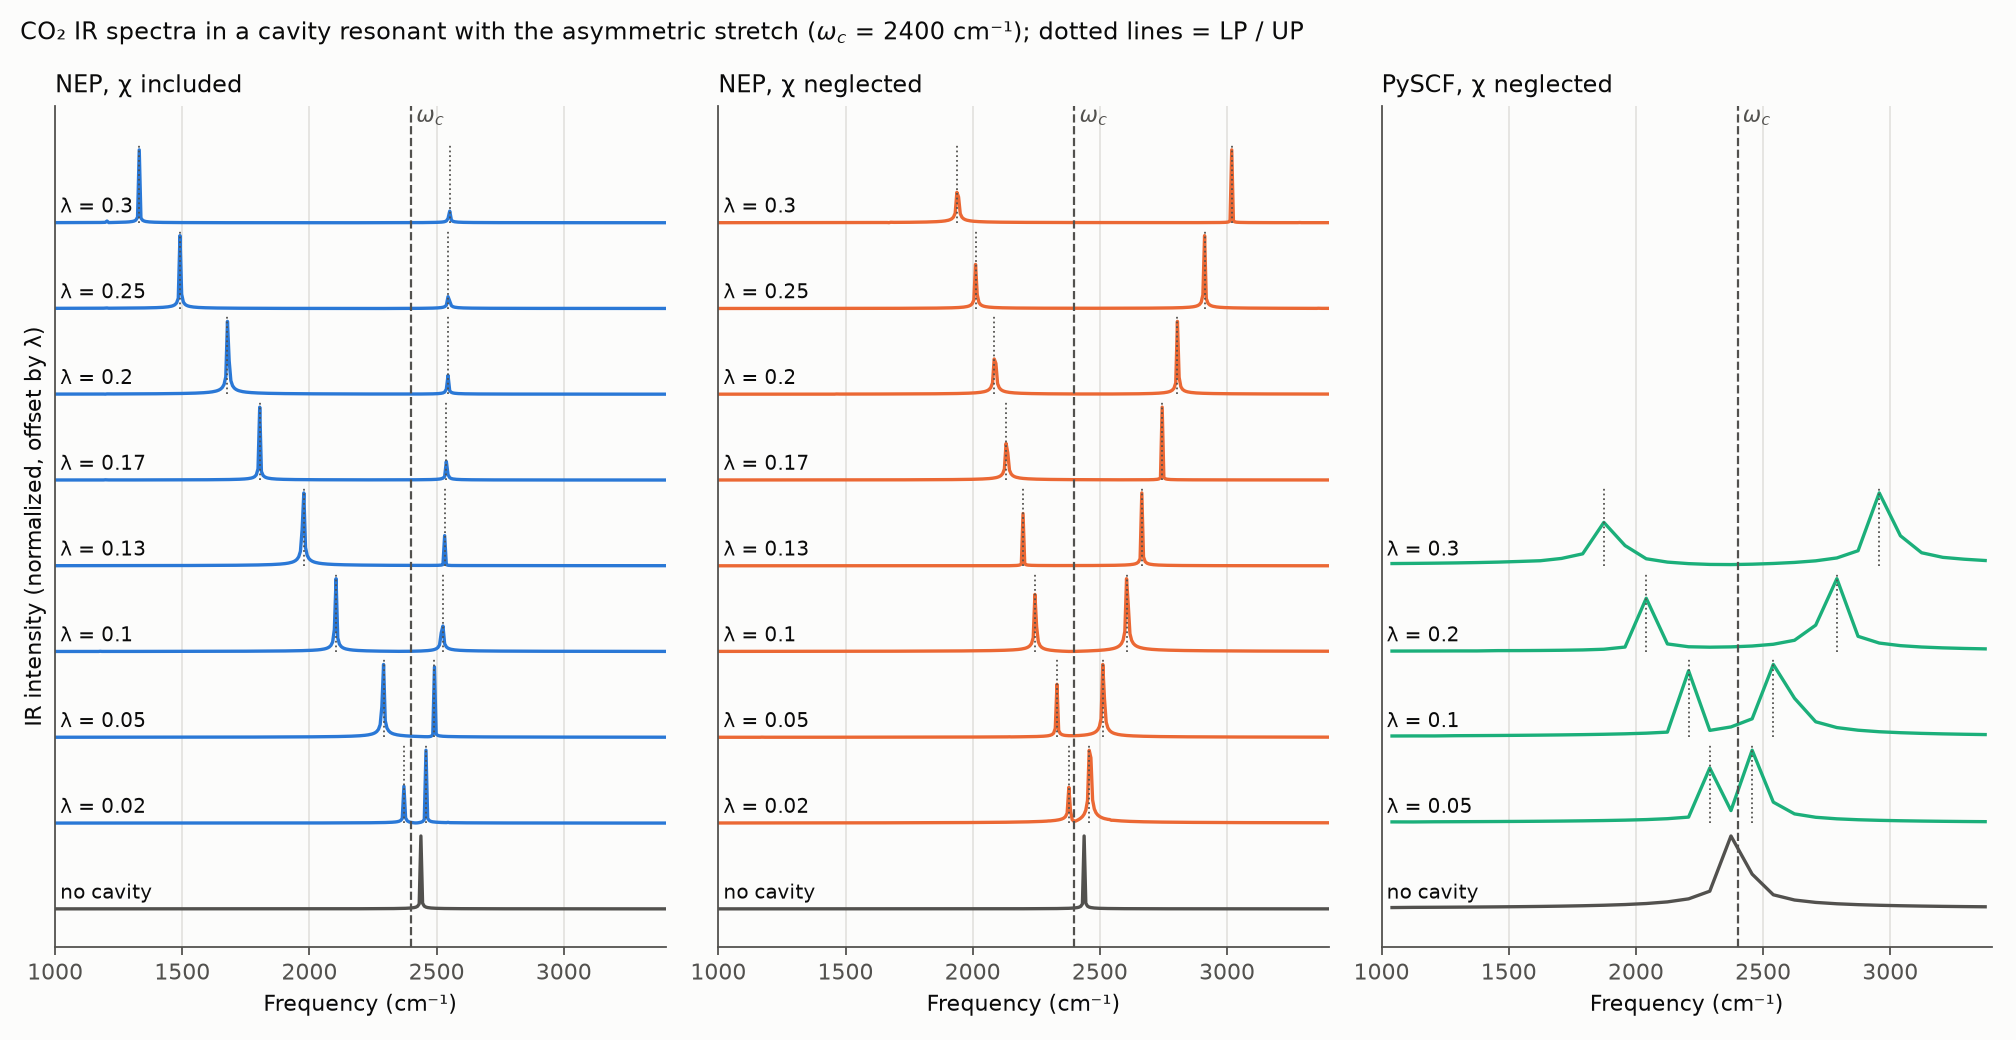
\includegraphics[width=\linewidth]{co2/2026-10-02_lambda_sweep/ir_spectra.png}
\caption{CO$_2$ IR spectra vs $\lambda$ (cavity at 2400~cm$^{-1}$). The asymmetric stretch
splits into LP and UP (dotted). With $\chi$ included, LP drops steeply and UP stays near
the bare mode. With $\chi$ neglected, the splitting is roughly symmetric. PySCF peaks are
broader because the runs are shorter (800 steps).}
\end{figure}

\begin{figure}[H]
\centering
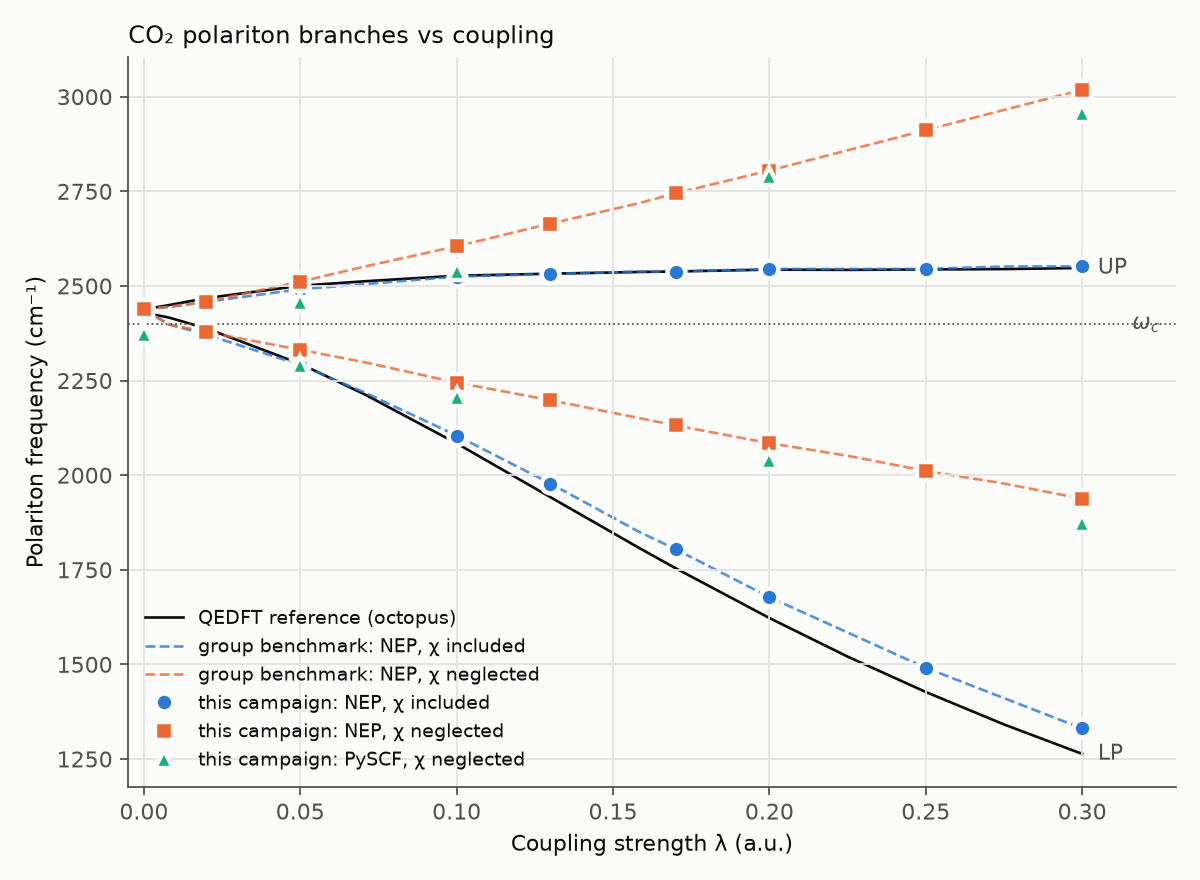
\includegraphics[width=0.49\linewidth]{co2/2026-10-02_lambda_sweep/polariton_branches.png}\hfill
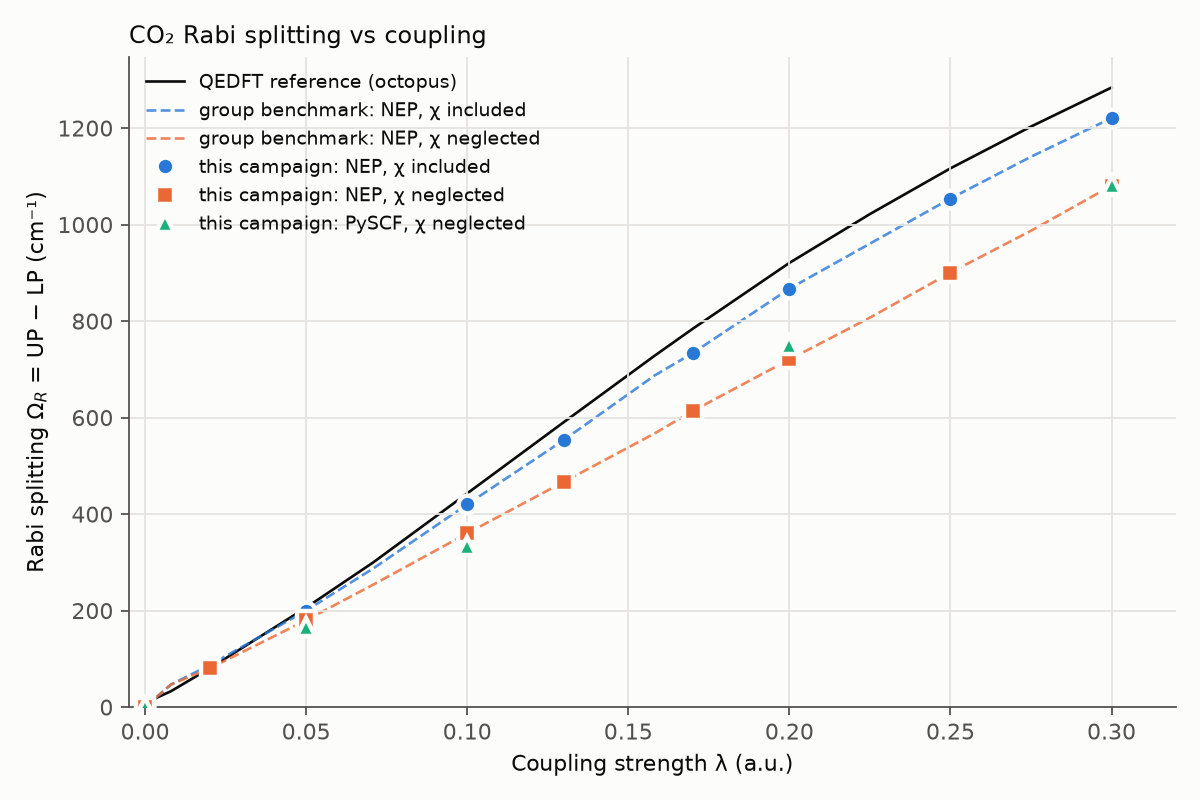
\includegraphics[width=0.49\linewidth]{co2/2026-10-02_lambda_sweep/rabi_splitting.png}
\caption{Left: CO$_2$ polariton branches. Right: Rabi splitting vs $\lambda$. Points are
this work, dashed lines are the group's NEP benchmark, and the solid line is the
explicit QEDFT reference (octopus).}
\end{figure}

\begin{table}[H]
\centering\small
\begin{tabular}{lcccc}
\toprule
$\Omega_R$ (cm$^{-1}$) at $\lambda$ = & 0.05 & 0.1 & 0.2 & 0.3\\
\midrule
NEP, $\chi$ included   & 200 & 420 & 867 & 1221\\
NEP, $\chi$ neglected  & 180 & 360 & 720 & 1081\\
PySCF, $\chi$ neglected & 167 & 333 & 750 & 1083\\
QEDFT reference        & 206 & 443 & 921 & 1284\\
\bottomrule
\end{tabular}
\end{table}

\textbf{Confirms:} the NEP points equal the group benchmark exactly, so the setup and
models are correct. PySCF matches NEP to within its 83~cm$^{-1}$ resolution. Including
$\chi$ raises $\Omega_R$ by about 15\% and brings it within about 5\% of QEDFT.

\section*{2. H$_2$O: $\lambda$ sweep}

\begin{figure}[H]
\centering
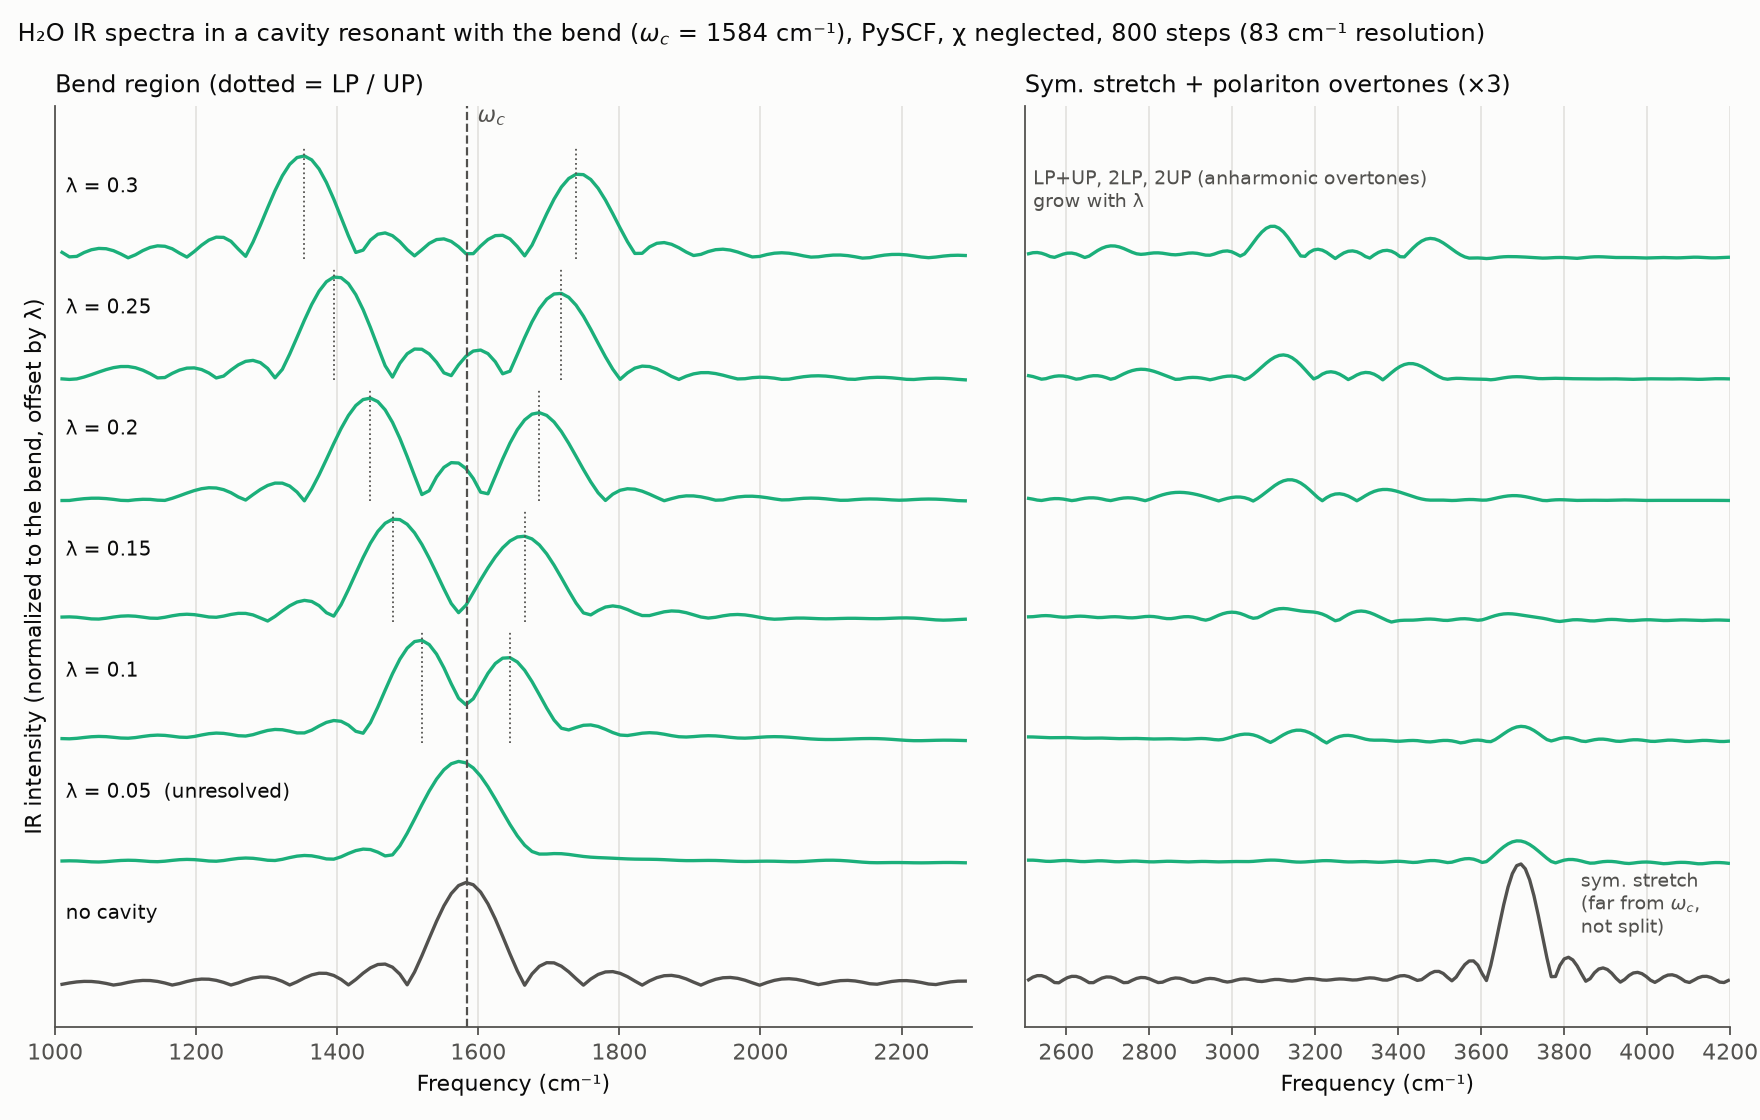
\includegraphics[width=\linewidth]{h2o/2026-10-02_lambda_sweep/ir_spectra.png}
\caption{H$_2$O spectra, $\chi$ neglected, with the cavity resonant with the bend
(1584~cm$^{-1}$). Left: the bend splits into LP and UP for $\lambda\ge0.1$ (not resolved
at $\lambda=0.05$). Right: weak LP+UP, 2LP and 2UP overtones appear as $\lambda$ grows.
The symmetric stretch is far detuned and doesn't split.}
\end{figure}

\begin{figure}[H]
\centering
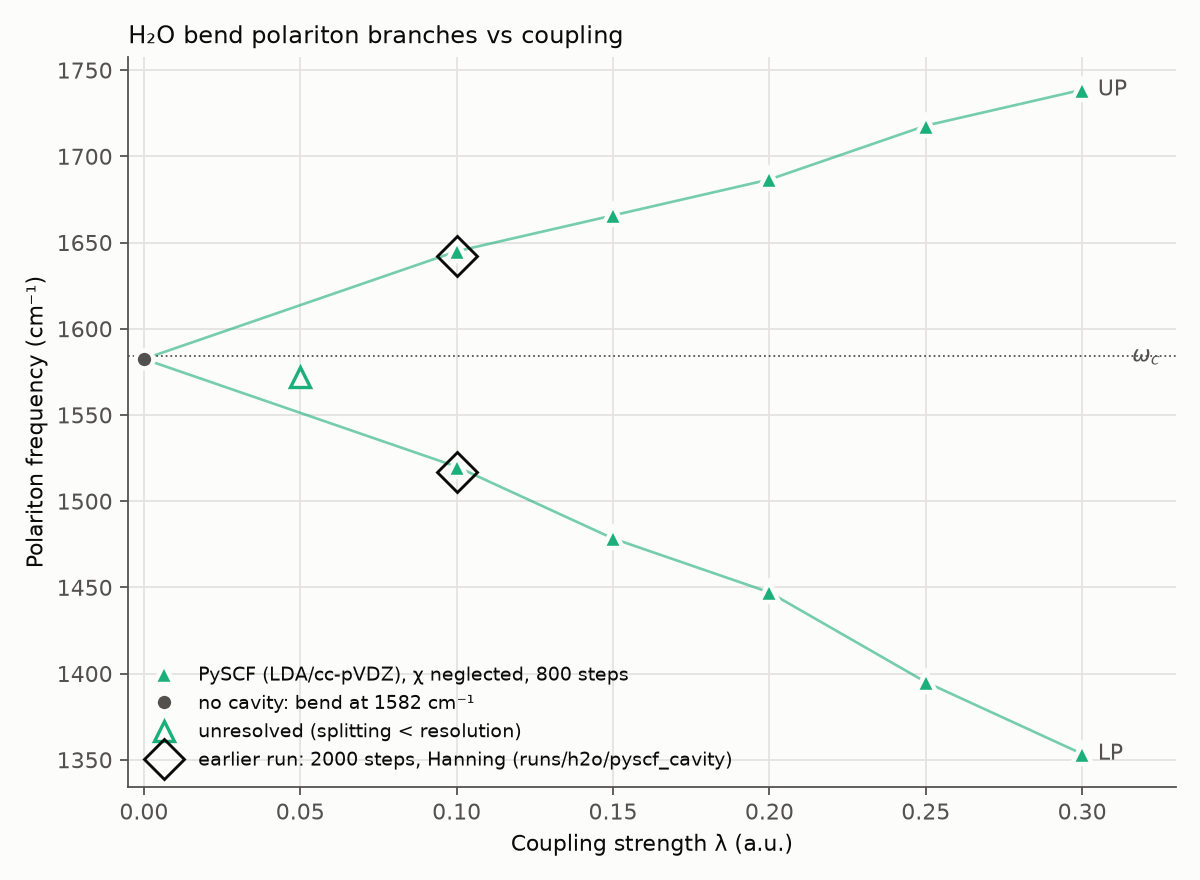
\includegraphics[width=0.49\linewidth]{h2o/2026-10-02_lambda_sweep/polariton_branches.png}\hfill
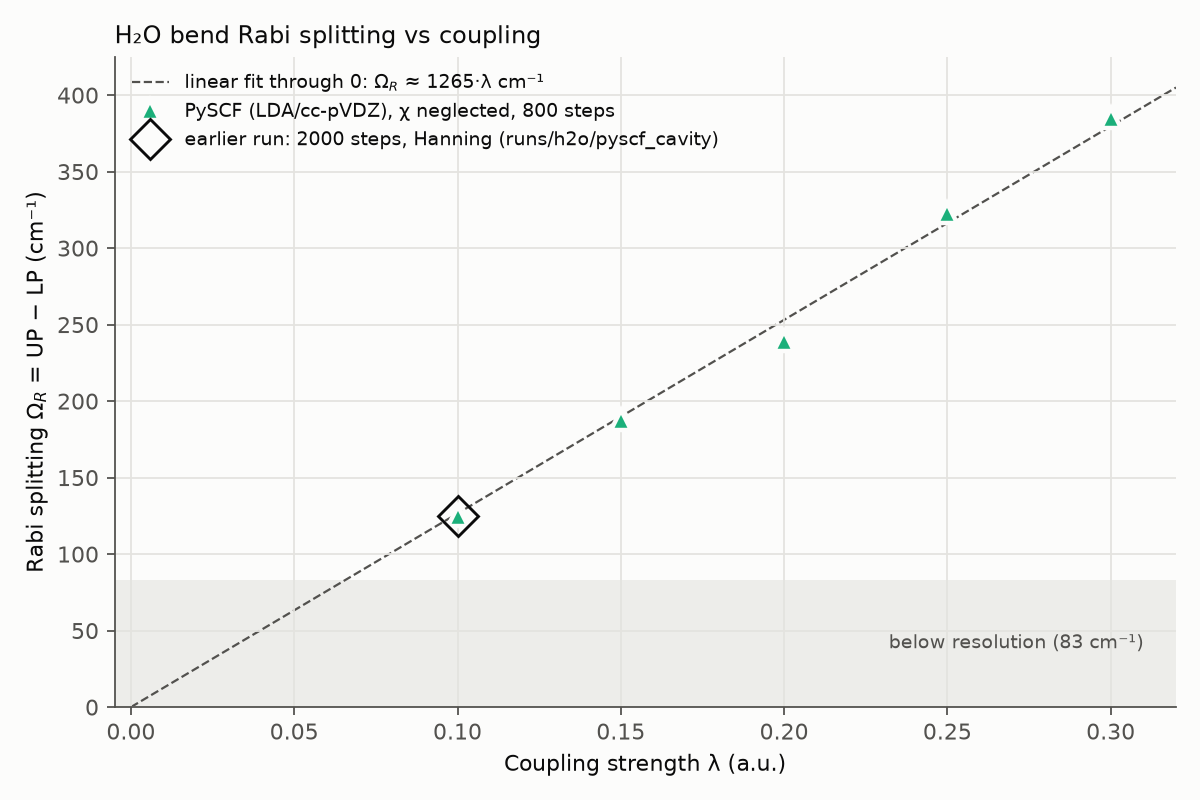
\includegraphics[width=0.49\linewidth]{h2o/2026-10-02_lambda_sweep/rabi_splitting.png}
\caption{Left: H$_2$O branches. Green is $\chi$ neglected. Orange is $\chi$ included,
dominant peak only, with the dotted line showing the screened cavity
$\omega_c/\sqrt{1+\lambda^2\chi_{xx}}$. Right: Rabi splitting ($\chi$ neglected) with a
linear fit. The diamond is the earlier 2000-step result.}
\end{figure}

\begin{table}[H]
\centering\small
\begin{tabular}{lccccc}
\toprule
$\lambda$ & 0.1 & 0.15 & 0.2 & 0.25 & 0.3\\
\midrule
$\Omega_R$, $\chi$ neglected (cm$^{-1}$) & 125 & 187 & 239 & 323 & 385\\
Dominant peak, $\chi$ included (cm$^{-1}$) & 1499 & 1437 & 1364 & 1291 & 1218\\
Screened cavity $\omega_c/\sqrt{1+\lambda^2\chi}$ (cm$^{-1}$) & 1541 & 1491 & 1429 & 1360 & 1286\\
\bottomrule
\end{tabular}
\end{table}

\textbf{Confirms:} with $\chi$ neglected, $\Omega_R$ is linear in $\lambda$, and
$\lambda=0.1$ reproduces the earlier 2000-step result (125~cm$^{-1}$). With $\chi$ included
($\chi_{xx}\approx5.7$~a.u.), the polarizability screens and red-detunes the cavity. One
polariton dominates and tracks just below the screened cavity frequency, the same
behaviour as the CO$_2$ $\chi$-included benchmark. The second polariton is weaker than
the finite-length side lobes at 800 steps, so there is no $\chi$-on $\Omega_R$ yet.

\section*{3. Single-molecule checks}

\textbf{Energy conservation.} All 67 runs conserve
$H = E_\text{kin} + E_\text{bare} + \tfrac12 p^2 + \tfrac12(1+\lambda^2\chi)\,e_a^2$ to
about 1\% (drift $<0.3\%$) at 0.5~fs, so no smaller timestep is needed. Note that
\texttt{md.log}'s $E_\text{tot}$ leaves out the cavity energy. Checked with
\texttt{scripts/check\_energy.py}.

\begin{figure}[H]
\centering
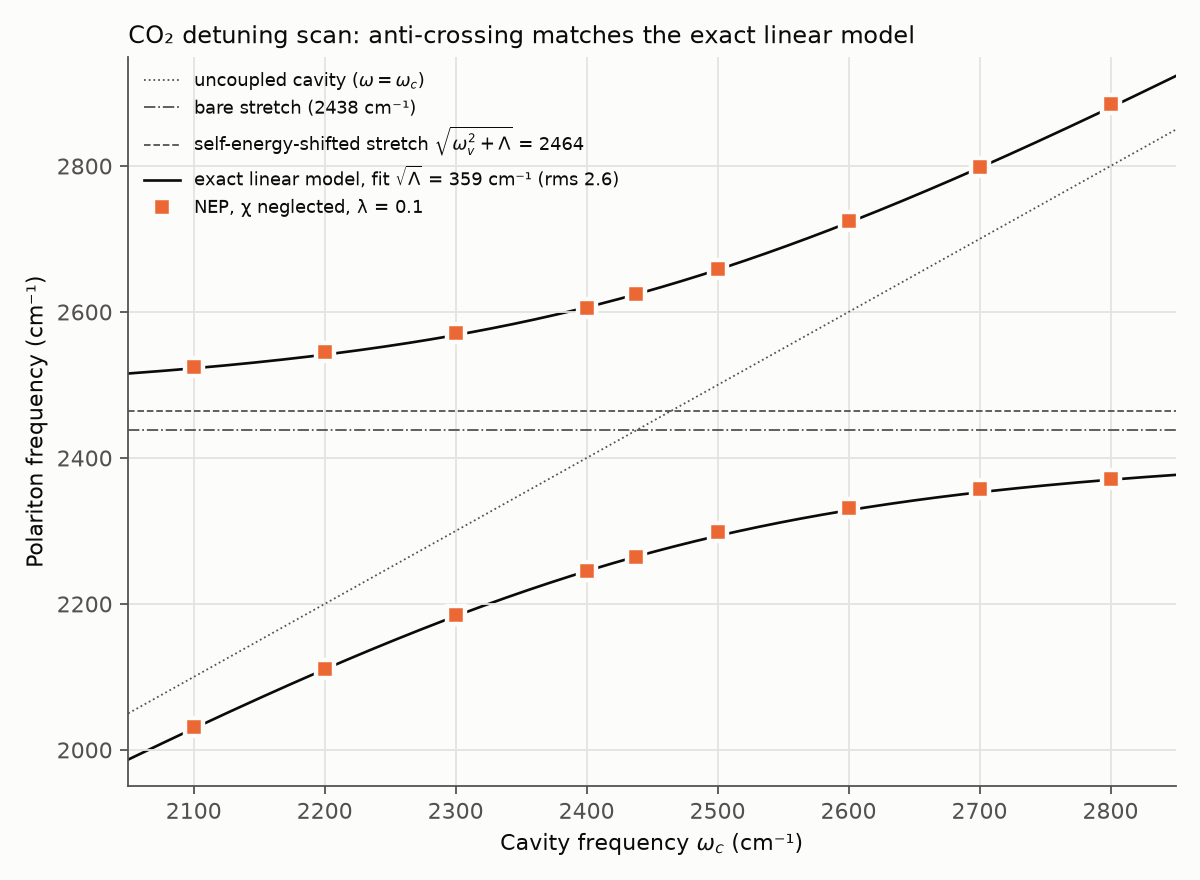
\includegraphics[width=0.49\linewidth]{co2/2026-10-02_checks/detuning.png}\hfill
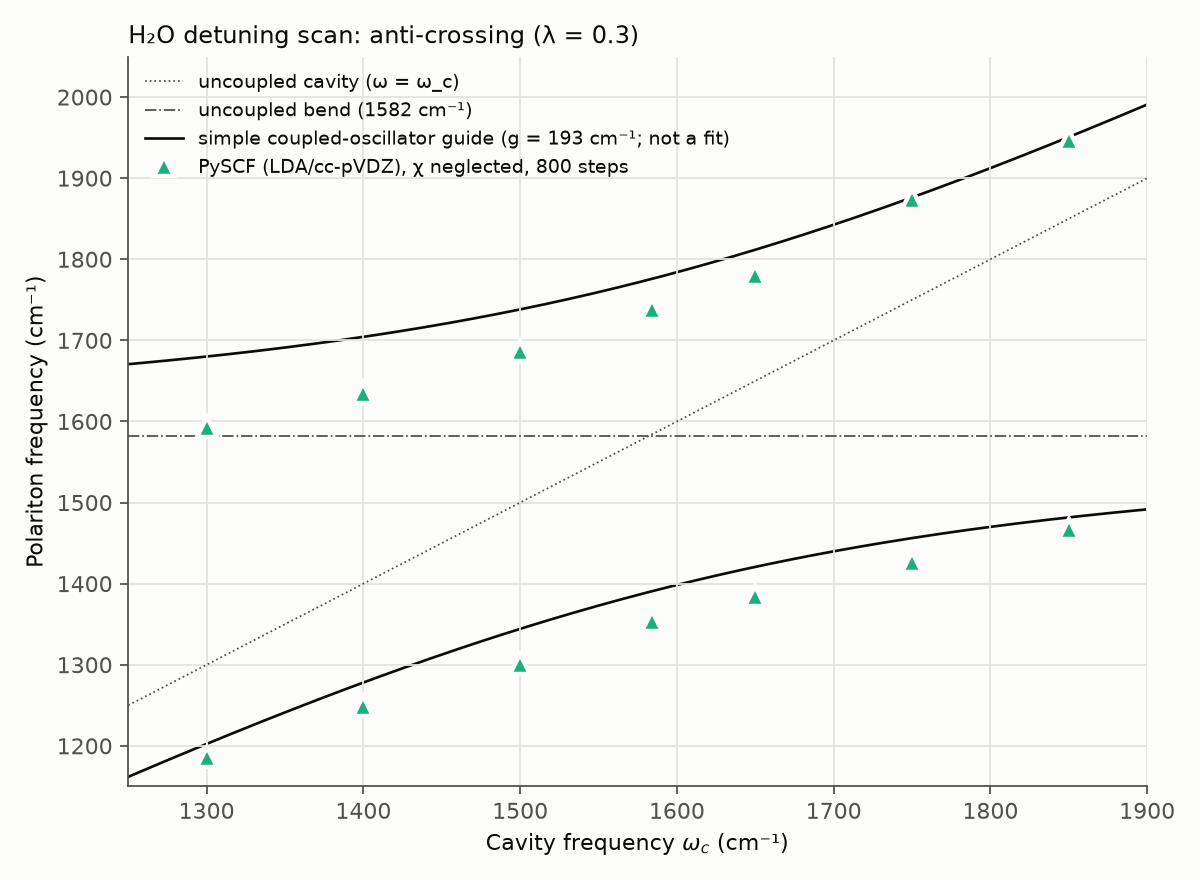
\includegraphics[width=0.49\linewidth]{h2o/2026-10-02_checks/detuning.png}
\caption{Detuning scans. Left: CO$_2$ (NEP, $\lambda=0.1$). The exact linear model
(vibration + cavity + dipole self-energy, one parameter) fits to 2.6~cm$^{-1}$ rms, and
the effective stretch is shifted to 2464~cm$^{-1}$. Right: H$_2$O (PySCF, $\lambda=0.3$).
There is a clear anti-crossing, but the points sit 40--60~cm$^{-1}$ below the simple model.}
\end{figure}

\begin{figure}[H]
\centering
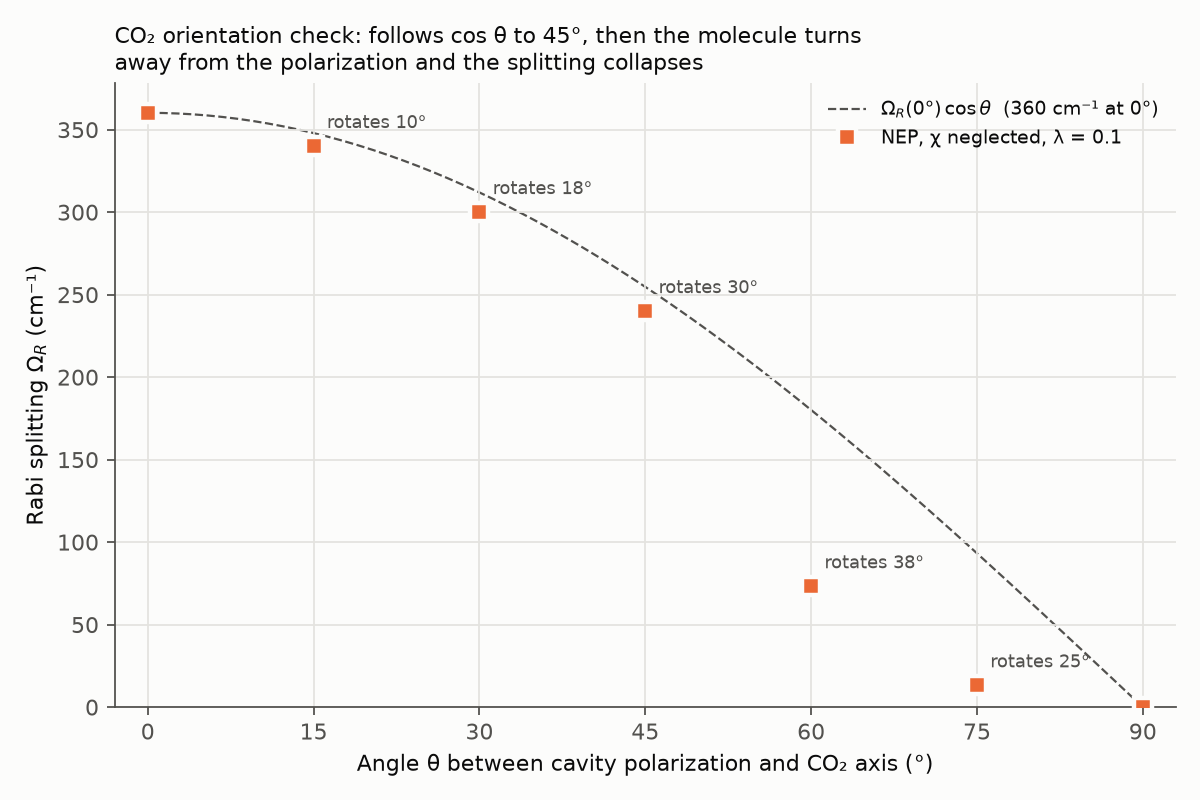
\includegraphics[width=0.49\linewidth]{co2/2026-10-02_checks/orientation.png}\hfill
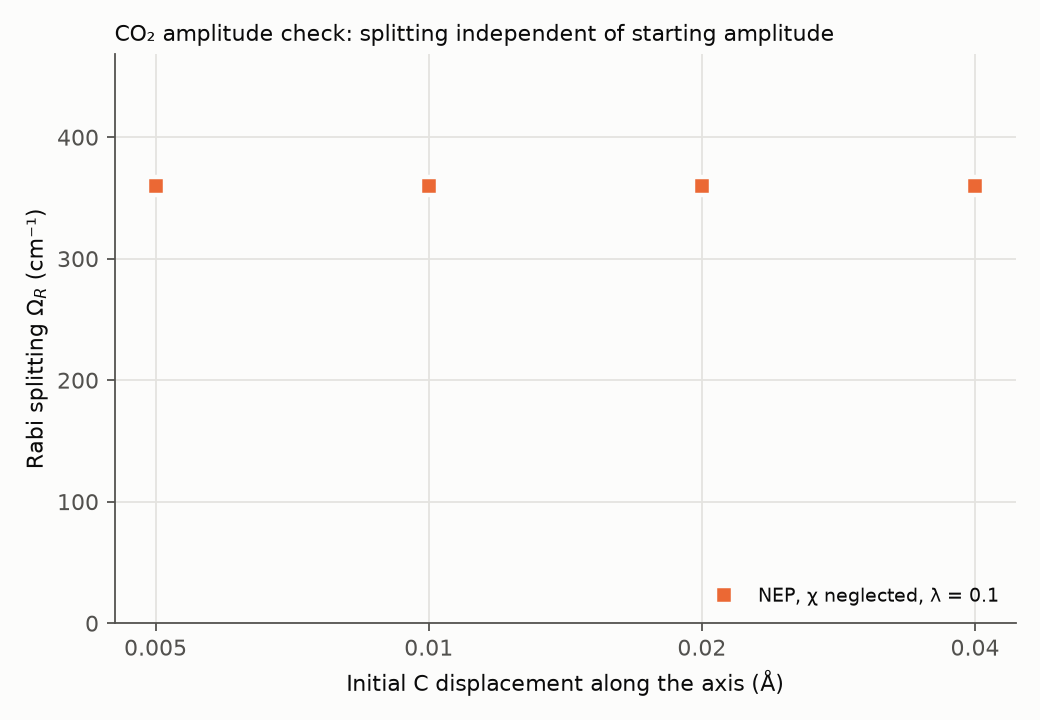
\includegraphics[width=0.49\linewidth]{co2/2026-10-02_checks/amplitude.png}
\caption{Left: CO$_2$ orientation. The polarization is tilted by $\theta$ from the
molecular axis. Right: CO$_2$ splitting vs initial displacement.}
\end{figure}

\textbf{Confirms:}
\begin{itemize}
  \item \emph{Amplitude:} $\Omega_R = 360$~cm$^{-1}$ for C displacements of 0.005--0.04~\AA,
        so the runs are linear and one trajectory per setting is enough.
  \item \emph{Detuning:} CO$_2$ behaves exactly like the textbook linear model. True
        resonance is near 2500~cm$^{-1}$, not the bare 2438, because of the dipole
        self-energy.
  \item \emph{Orientation:} CO$_2$ follows $\cos\theta$ to about 5\% up to $45^\circ$.
        Beyond that, the molecule rotates away from the polarization (10--38$^\circ$) and
        $\Omega_R$ collapses. H$_2$O, which has a permanent dipole, rotates even more
        (49$^\circ$ at $\theta=30^\circ$, 113$^\circ$ at $60^\circ$), so it gave no clean
        $\cos\theta$ test.
\end{itemize}

\section*{Next steps}

\begin{enumerate}
  \item H$_2$O with $\chi$ on in the ``resonant'' variant
        ($\omega_c \to \omega_c\sqrt{1+\lambda^2\chi}$), or with longer runs plus a
        window, to resolve both polaritons.
  \item Settle orientation and rotation (questions below) before choosing a 2--3 molecule
        geometry.
  \item First multi-molecule test: 2--3 H$_2$O (PySCF), well separated ($>10$~\AA) and
        aligned with the cavity, to check $\Omega_R \propto \sqrt{N}$ against the
        single-molecule slope.
\end{enumerate}

\section*{Questions}

\begin{enumerate}
  \item Is the molecular rotation in a tilted cavity field expected? Should orientation
        be fixed, or coupling kept lower, for multi-molecule runs, or is rotation part of
        the physics we want?
  \item Should multi-molecule runs use $\chi$ with the resonant (un-screened)
        $\omega_c$, as in \texttt{nep\_chi\_resonant}?
  \item Which analytic model applies to the e-mode for a polar molecule? The H$_2$O
        detuning offset doesn't fit the linear dipole-self-energy model that works for CO$_2$.
  \item Is the CO$_2$ NEP model valid for CO$_2$ pairs and clusters, or only single molecules?
\end{enumerate}

\vfill
{\small Data, scripts and figures: \texttt{github.com/charliew0707/VSC\_Molecular\_Dynamics}.
Campaign scripts are in \texttt{scripts/campaigns/}, plot scripts in \texttt{scripts/plot\_*.py},
and peak tables in \texttt{results/*/*/peaks.csv}.}

\end{document}
